
\chapter{基于动态词向量的联合嵌入模型}
视觉问答来的研究受到机器学习算法在自然语言处理和图像识别等领域成功应用的启发,因此从2015年视觉问答任务出现至今,大量的VQA模型都使用了联合嵌入模型,使之成为目前视觉问答的的主流模型。顾名思义,联合嵌入模型是将任务的源信息——图像和问题文本——表示为向量,再通过特征融合,将不同模态的信息映射到统一的向量空间,最终从联合表征中提取出答案。因为这种架构的模型易于训练,研究者采用不同的图像特征的提取方法、不同的文本特征的提取方法、两种模态的不同融合方法,做了许多尝试。

Antol等人在2015年发布了开放问题的视觉问答数据集VQA\citing{antol2015vqa}之后,在数据集的基础上提出了VQA挑战。VQA挑战中涌现了大量视觉问答模型,模型的准确率也逐年升高,图\ref{vqa_challenge}展示了2015年-2019年VQA挑战中的最优模型的准确率。通过研究其中表现优异的模型,我们发现几乎所有模型都使用了联合嵌入模型,并且加入注意力机制之后准确率能够进一步提升,例如,四年的冠军模型都是使用了注意力机制的联合嵌入模型,其中2019年的冠军模型\citing{Yu_2019_CVPR}能在VQA2.0数据集下获得总体75\%作用的准确率,相较于四年前的模型准确率得到了20\%的提升,并且距离人类表现也只有5\%左右的差距。
\begin{figure}[H]
	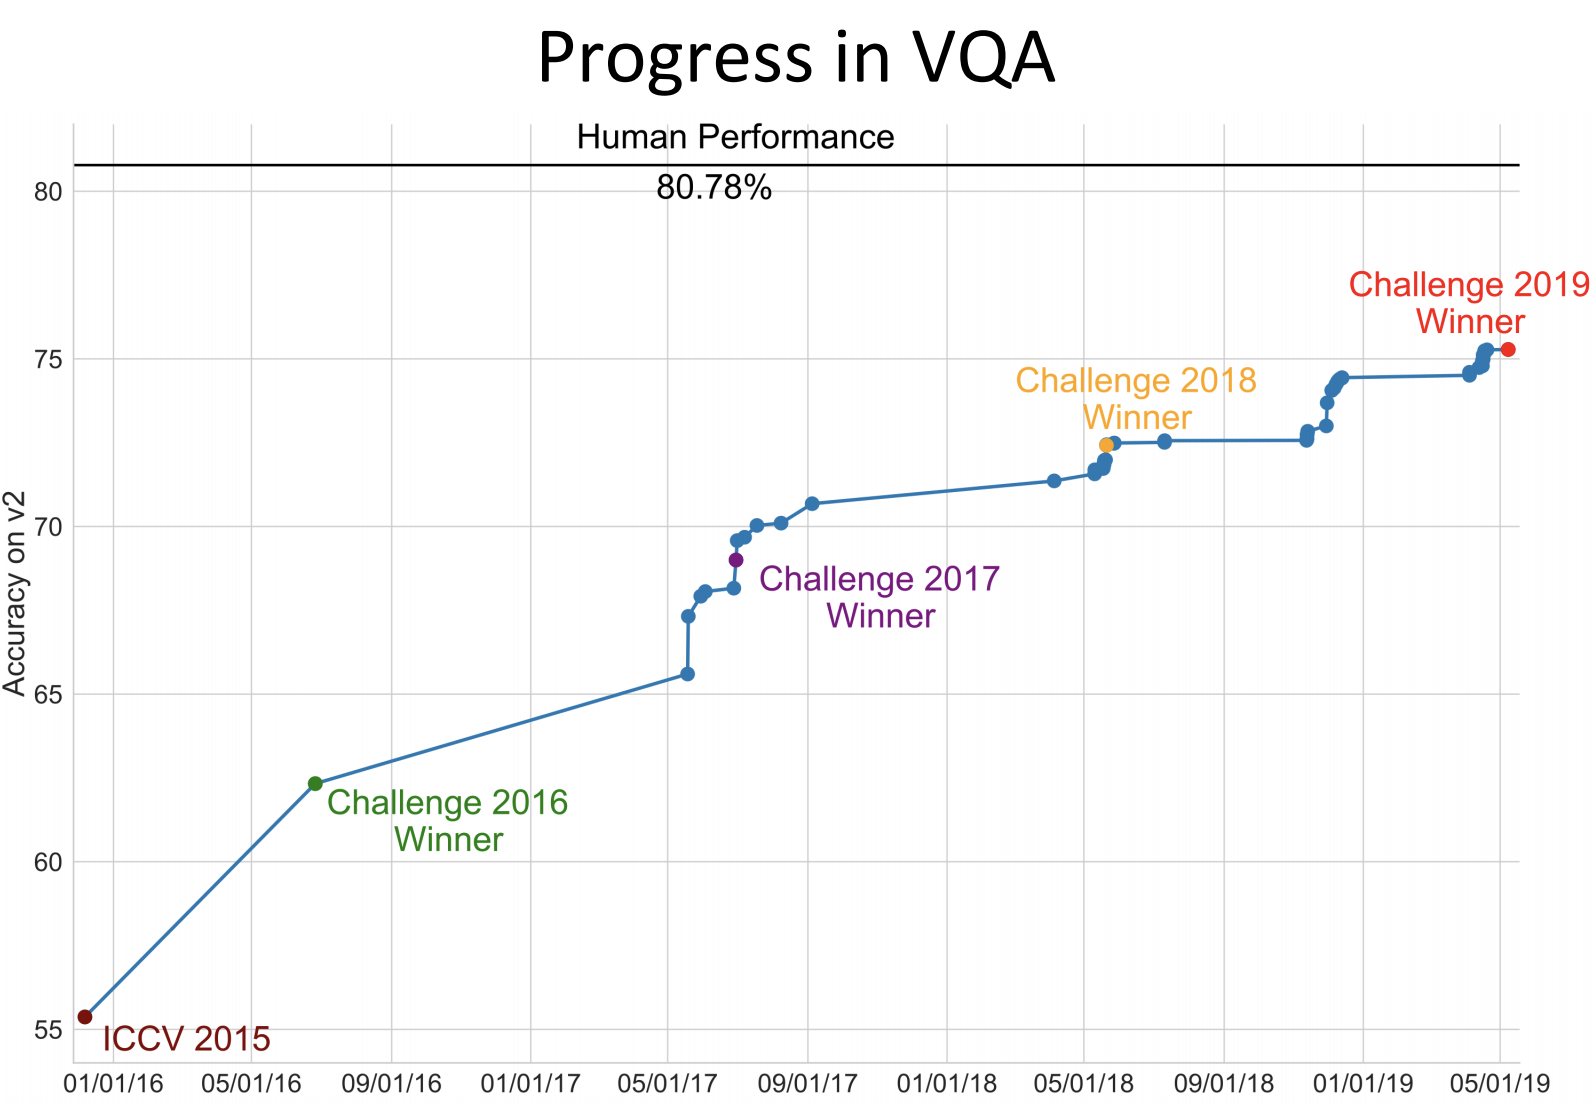
\includegraphics[width=0.7\textwidth]{vqa_challenge.png}
	\caption{视觉问答模型在VQA挑战的准确率曲线,其中四年的优胜模型都是使用联合嵌入模型。}
	\label{vqa_challenge}
\end{figure}

我们认为联合嵌入模型在VQA挑战的优异表现有以下几点原因。
\begin{itemize}
  \item [1)] 
  引入注意力机制。2016年的优胜模型\citing{ilievski2016focused}提出“动态关注注意力(FDA)”模型,目的是根据问题中的关键词动态的对图像的不同区域分配带有权重的注意力,得到图像的全局特征和局部特征的结合。2017和2018年的优胜模型都使用论文\citing{anderson2018bottom}中的自上而下和自下而上的图像注意力机制,2019年的优胜模型使用了Transformer\citing{NIPS2017_7181}的多头注意力机制。注意力机制的引入能够减少无关特征的干扰,提高计算效率,并且一定程度的提高可解释性。
  \item [2)]
  VQA2.0数据集的局限性。VQA挑战以VQA2.0为数据集,然而根据我们提出的依照答案和源信息统计相关性的标准(详见表\ref{ques_type}),VQA2.0中需要常识或者外源知识的qi类型仅仅占所有问题的5.5\%\citing{wang2015explicit},这意味着回答绝大多数的问题都不需要额外的信息。然而在现实中的开放性问题中,涉及常识或者外源知识的问题广泛存在,因此VQA2.0数据集存在局限性,而这种局限性使得模型只需要关注图像和文本,因此联合嵌入模型成为了主要架构。
  \item [3)]
  得益于图像识别和自然处理模型的进步。联合嵌入模型具有灵活的组合模式,很容易从将其他任务中表现优异的模型迁移过来形成新的模型。
\end{itemize}

在本文的研究中,为实现一个通用的VQA架构,我们分成两个阶段完成,第一部分是沿袭联合嵌入模型的思路,构建一个基于动态词向量的联合嵌入模型——None KB-Specific Network(N-KBSN)模型,该模型仅仅使用图像特征和文本特征,不使用外源知识。第二个阶段是在N-KBSN模型的基础上,融合知识库的图嵌入,提出KB-Specific Network(KBSN)模型。

本章将重点介绍N-KBSN模型,并且使用VQA2.0数据集训练。N-KBSN由三个主要部分组成:问题文本和图像特征提取模块、自注意力和引导注意力模块、特征融合和分类器。其中,图像特征提取使用在多目标检测中表现优秀的Faster R-CNN\citing{ren2015faster},问题文本特征提取使用能够获得上下文信息的ELMo模型\citing{Peters:2018},并使用从Transformer中借鉴的多头注意力机制\citing{NIPS2017_7181}分别实现图片的自注意力(V-SA)、问题文本的自注意力(Q-SA)、由问题引导的对图像的注意力(Guided Attention, GA),最后通过特征融合预测答案。N-KBSN模型的基础架构如图\ref{N-KBSN}。
\begin{figure}[H]
	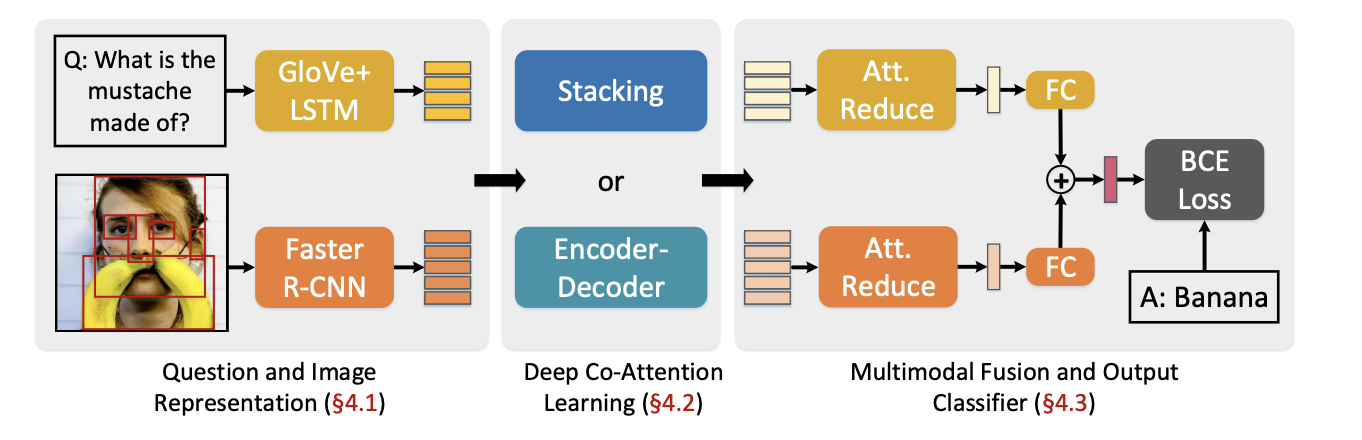
\includegraphics[width=0.8\textwidth]{N-KBSN.png}
	\caption{N-KBSN基础结构}
	\label{N-KBSN}
\end{figure}

\section{基于Faster R-CNN的图像特征化}
目标检测是机器视觉领域的重要应用之一,目标检测的核心任务是准确、快速的从图像中定位出目标并且能识别目标的类别、属性等特性。在 2012 年深度学习正式介入计算机视觉目标检测任务之前,传统的目标检测算法一直是以滑动窗口卷积等较为传统的方式进行区域选择、特征提取和分类回归等步骤,例如可变形的组件模型(DPM)方法\citing{felzenszwalb2009object}等。这些传统的目标检测算法大多区域选择的策略效果差、时间复杂度高,并且因为由于是人工提取特征,提取的特征层次较低,致使模型的鲁棒性较差。在深度学习兴起并逐渐成为计算机视觉的核心方法之后,大批优秀的目标检测算法出现,例如R-CNN\citing{girshick2014rich}、SPP-Net\citing{he2015spatial}、Fast R-CNN\citing{girshick2015fast}、Faster R-CNN\citing{ren2015faster}、Mask R-CNN\citing{he2017mask}、YOLO\citing{redmon2016you}及其后续版本等。以上的模型大致分为两个主要类别,第一类为两级式检测框架,包含一个用于区域提议的预处理步骤,使得整体流程是两级式的,例如一系列的R-CNN模型;第二类为单级式检测框架,即无区域提议的框架,这是一种单独提出的方法,不会将检测提议分开,使得整个流程是单级式的,例如YOLO系列的模型。由于Faster R-CNN在各个目标识别任务的出色表现,本节将省略对单级式检测框架的介绍,并着重介绍本文中图像处理的核心模型Faster R-CNN。

区别于传统的滑动卷积窗口来判断目标的可能区域,R-CNN 采用选择性搜索的方法来预先提取一些可能包含目标物体的候选区域(region proposal),再使用卷积神经网络提取各个图像区域的特征,再将提取的特征送入SVM分类器完成类别识别,最后使用回归器对目标位置进行修正。这种方法显著的提升识别速度,降低了计算成本,也提高了准确率。因为R-CNN需要分别对每一个生成的候选区域进行一次特征提取,存在着大量的重复运算,制约了算法性能。为了减少R-CNN的重复计算,研究者提出了SPP-Net。该算法通过在网络的卷积层和全连接层之间加入空间金字塔池化层(Spatial Pyramid Pooling)来对利用 CNN 进行卷积特征提取之前的候选区域进行裁剪和缩放使 CNN 的输入图像尺寸一致。随后的Fast R-CNN借用了SPP-Net的空间金字塔池化层,设计了兴趣区域池化(RoI Pooling),将图像中的多个兴趣区域池化成相同大小的特征图,并使用这些特征图同时预测物体类别和框出对象的区域。这种方法解决了输入候选区域尺寸不一致的问题,并且提高了计算速度。但是Fast R-CNN在生成生成候选区域的较慢,为了解决这一问题,R-CNN的作者又提出了Faster R-CNN。

Faster R-CNN同样沿袭了先前R-CNN和Fast R-CNN的两级式检测框架,但是为了解决之前的大量候选框导致的速度慢的问题,Faster R-CNN设计了一个用于选择和判断候选区域的网络(Region Proposal Network, RPN),该网络将CNN处理后的全局图像特征作为输入,输出候选区域,最终的分类器结合全局的图像特征和候选区域预测各个区域的类别。
\begin{figure}[H]
	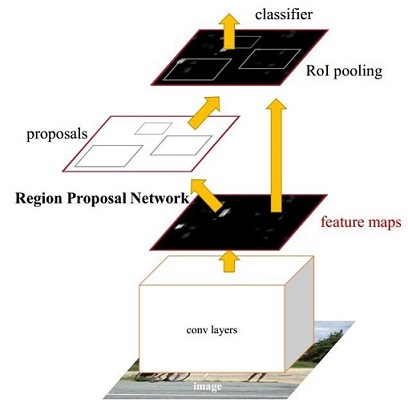
\includegraphics[width=0.5\textwidth]{Faster_R_CNN.png}
	\caption{Faster R-CNN基本结构}
	\label{Faster_R_CNN}
\end{figure}

如图\ref{Faster_R_CNN},Faster R-CNN可以根据功能的不同将模型分为四个模块:卷积层、区域候选网络(RPN)、兴趣区域池化(RoI Pooling)、分类器。卷积层使用CNN及其变型提取图像特征,生成的特征图被共享用于后续RPN层和全连接层,这种对图像的处理方式不同于R-CNN和Fast R-CNN。后两者都是先从原始图像中提取候选区域,再分别对候选区域提取特征。RPN网络用于预测候选区域,该网络在CNN输出的图像特征上滑动,在每个空间区域,网络都会预测类别得分,通过softmax判断锚点(anchors)属于前景(foreground)或者背景(background),利用候选框回归(bounding box regression)修正锚点获得精确的候选区域。兴趣区域池化层收集输入的特征图和候选区域,综合这些信息后提取候选区域特征图,送入后续全连接层判定目标类别。分类器利用候选区域特征图计算区域的类别,同时再次使用候选框回归获得检测框最终的精确位置。

在本文中,我们使用联合在ImagNet\citing{russakovsky2015imagenet}上预训练的ResNet-101和在Visual Genome\citing{krishna2017visual}上预训练Faster R-CNN提取图像特征。给定图像$I$,我们从图像中提取$m$个大小不固定的图像特征,$X=\{x_1, x_2, ..., x_m\}, x_i \in \mathbb{R}^D$,每一个图像特征编码一个图像区域。对卷积层输出的特征图,使用非极大抑制(non-maximum suppression)和单元重合(IoU)阈值筛选出排名靠前的候选区域,通过设定一个目标检测概率的阈值,我们获得一个动态的被检测对象的数量$m \in [10,100]$,并且使用零填充使得$m=100$。对于每个所选区域$i$,$x_i$被定义为该区域的特征图的均值池化结果,并将$m$个区域的$x_i$拼接成为最终的图像特征。

\section{基于ELMo的文本特征化}
和众多自然语言处理任务一样,在视觉问答任务中如何准确理解问题内容对最终的答案准确率上有着决定性的影响。而自然语言理解中最为基本和核心的便是文本表达,文本表达将自然语言转换为计算机可处理的数字,为自动化处理文本相关的任务建立了基础。在文本表达中,独热向量(one-hot)是最早也是最为简单的词向量。但是其稀疏性会带来的“维度灾难”和因简单的编码方式而造成“语义鸿沟”。基于分布式假设——即处于相似上下文的词语具有相似的含义,研究者先后提出了多种使用分布式表示的词向量模型,例如,CBOW,Skip-Gram,word2vec\citing{mikolov2013distributed},潜在语义分析(LSA)\citing{landauer1998introduction},GloVe\citing{pennington2014glove},ELMo\citing{Peters:2018},BERT\citing{DBLP:journals/corr/abs-1810-04805}等。

CBOW和Skip-Gram均是使用神经网络模型训练上下文信息得到词向量。word2vec也使用了CBOW与Skip-Gram来训练模型与得到词向量,但是并没有使用传统的DNN模型,而是使用霍夫曼树来代替隐藏层和输出层的神经元,提高了计算效率,因此被研究者广泛地使用作为预训练的词向量。但是由于word2vec使用滑动窗口来限定上下文信息,因此得到的词向量仅仅使用了局部的语义和语法信息。不同于word2vec使用局部语料,潜在语义分析(LSA)采用统计计数的方式获得语料的全局信息,其统计预料库中每两个词共同出现的次数构成共现矩阵,并采用了基于奇异值分解(SVD)的矩阵分解技术对大矩阵进行降维,得到词向量。然而LSA方法中的SVD计算量很大,并且共现矩阵仅能表示两个词语同时出现的次数,并不能表示词语之间的远近关系。为了改进word2vec的局部预料限制和LSA的计算复杂性,GloVe使用衰减函数改造LSA的共现矩阵,使得词语间的远近关系得以表达。GloVe还构建了词向量和共现矩阵之间的近似关系,使用梯度下降算法取代了LSA中的奇异值分解,大大减少了计算代价,并且得到了远超LSA和word2vec的性能。

以上提到的所有模型都是通过对语料库的学习得到静态的词向量,即每个单词对应一个确定的实数向量,这种固定向量在处理词汇的多义性上表现不佳。无论是中文词语还是英文单词都广泛得存在一词多义的现象,即同一个词在不同的语境下含义发生变化,例如,在中文中,“他正在算账”和“下回找你算账”中的“算账”由于文化演化而产生了更复杂的引申义,又如英文中的“where is the bank?”和“It is the bank of the river”中的“bank”在第一句中译为“银行”而第二句中译为“河畔”。为解决一词多义的问题,研究者提出了动态词向量,ELMo和BERT便是其中的代表。ELMo在多个NLP任务中均提高了模型的准确率,因此本文将着重介绍并使用ELMo模型处理视觉问答任务中的文本,并在后续的处理中结合类似于BERT的注意力机制。

ELMo是一种深度场景化的词表示。其模型深度能够对复杂的词语使用特性——语法和语义特征进行有效建模,而其模型的动态性能根据词语的上下文的不同生成动态向量,进而为解决一词多义提供了可能。ELMo采用了两个阶段获得词向量,第一个阶段是用大量的文本语料训练一个深度双向语言模型(biLSTM);第二个阶段从预训练网络中提取对应单词的网络各层的内部状态(internal state),并通过函数转化为词向量。ELMo模型的结构如图\ref{elmo}。
\begin{figure}[H]
	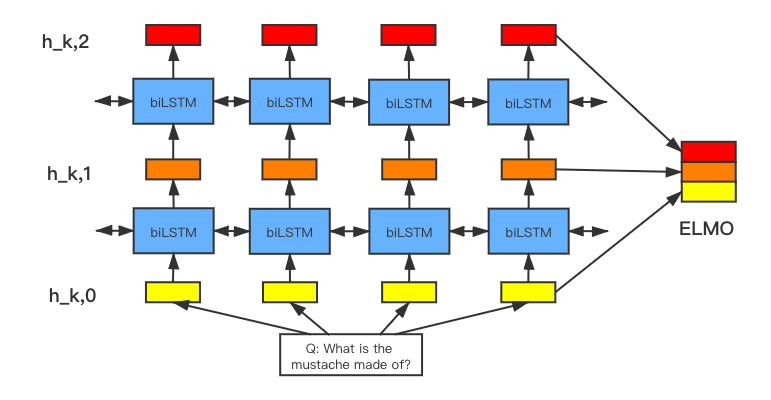
\includegraphics[width=0.8\textwidth]{elmo.png}
	\caption{ELMo使用两层的biLSTM层,并对每一层的输出加权得到词嵌入。}
	\label{elmo}
\end{figure}

语言模型是对语句的概率分布的建模。语言模型分为前向和后向,前向是指已知上文的词语,推理下一个词语的方式,而后向则是已知后文的内容,求解上一个词语的方式。对于一个具有N个单词的句子$S=(t_1, t_2, ..., t_N)$而言,前向语言模型就是求解以下公式的最大值:
\begin{equation}
p(t_1, t_2, ..., t_N)=\prod_{k=1}^N p(t_k|t_1,t_2,...,t_{k-1})
\end{equation}
其中$p(t_1, t_2, ..., t_N)$为序列的联合概率,
$p(t_k|t_1, t_2,..., t_{k-1})$表示已知$t_k$的上文$(t_1, t_2, ..., t_{k-1})$的条件下,求解$t_k$的条件概率。对应的后向语言模型的公式为
\begin{equation}
p(t_1, t_2, ..., t_N)=\prod_{k=1}^N p(t_k|t_{k+1},t_{k+2},...,t_N)
\end{equation}

ELMo使用双向LSTM(biLSTM)模型作为语言模型的基础。首先将“上下文无关的”初始词向量$y{_k^{LM}}$输入L层的前向LSTM。在位置k上,LSTM将输出一个“上下文相关”的词表征$\vec{h}_{k,j}^{LM,j}$,其中$j = 1, ..., L$。最后一层的LSTM输出$\vec{h}_{k,j}^{LM,L}$通过一个softmax层预测下一个词语的初始词向量$y{_{k+1}^{LM}}$。后向LSTM类似于前向LSTM有L层并且在k位置上得到一个词表征$\overleftarrow{h}_{k,j}^{LM}$。最后通过最大似然的方式训练双向LSTM模型,公式如下:
\begin{equation}
\sum_{k=1}^N(\log_p(t_k|t_1, t_2,..., t_{k-1};\Theta_x,\overrightarrow{\Theta_{LSTM}},\Theta_s) + \log_p(t_k|t_{k+1},t_{k+2},...,t_N;\Theta_x,\overleftarrow{\Theta_{LSTM}},\Theta_s)
)
\end{equation}

其中,$\Theta_x$和$\Theta_s$分别是初始词向量训练时的两个softmax层参数,$\overrightarrow{\Theta_{LSTM}}$和$\overleftarrow{\Theta_{LSTM}}$则是双向语言模型的参数。

当完成预训练阶段后,向网络输入一个新句子,句子中每个单词都能得到对应的三种Embedding:最底层是初始的词向量$y{_k^{LM}}$;前向LSTM输出的$\overrightarrow{h}_{k,j}^{LM}$;后向LSTM输出的$\overleftarrow{h}_{k,j}^{LM}$。ELMo将三种词向量串联,得到
\begin{equation}
R_k = 
[y_k^{LM}, \overrightarrow{h}_{k,j}^{LM}, \overleftarrow{h}_{k,j}^{LM} | j = 1, ..., L]
= [h_{k,j}^{LM} | j = 0, ..., L]
\end{equation}

其中$h_{k,0}^{LM}$是初始词向量,$h_{k,j}^{LM} = [\overrightarrow{h}_{k,j}^{LM}; \overleftarrow{h}_{k,j}^{LM}]$ 是每个biLSTM层输出的结果。

最后使用以下公式得到对应单词的具有”上下文信息“的词向量。
\begin{equation}
ELMo_k^{task} = E(R_k; \Theta^{task}) = \gamma^{task}\sum_{j=0}^L s_j^{task} h_{k,j}^{LM}
\end{equation}

其中是$s_j^{task}$任务相关训练得到的权重参数, $\gamma$是一个任务相关的scale参数。

在本文中,我们将句子最大长度裁剪为14个,并使用零填充的方式将不足14个词的句子补足为14,即$n=14$。并将每个单词转化为50维的初始词向量,即$y_k^{LM}\in \mathbb{R}^{50}$。假定双向语言模型的层数为$L = 2$,隐层节点数为$H_{dim}$,输出维度为$output_{dim} \in \mathbb{R}^d$,则$ELMo_k^{task} \in \mathbb{R}^{2d}$,输出的文本特征$Y \in \mathbb{R}^{n\times 2d}$。

\section{基于多头注意力机制的特征增强}
正如绪论中提到的,注意力机制的引入帮助神经网络提高了预测精度,并且减少了计算复杂度。视觉问答任务由于需要处理多模态的数据——图像和文本,比起仅需要处理单模态的数据的任务更需要进行高效的计算。同时,VQA任务输入的图像和问题文本具有高度的相关性,因此两种模态的数据之间的交互对于结果的准确性的提升也具有显著的影响。对于以上两个需求,我们在N-KBSN中使用了Transformer\citing{NIPS2017_7181}的多头注意力机制(Multi-head Attention, MA)实现图片的自注意力(V-SA)、问题文本的自注意力(Q-SA)、由问题引导的对图像的注意力(Guided Attention, GA)。

注意力机制本质上是找到一个方式对已有信息分配合适的权重,并以此提高输出的准确性。我们可以将注意力函数描述成映射查询(query)到一些键值对(key-value pair)并由此得到输出。假定查询矩阵$Q = \{q_1, q_2, ..., q_m\}$,其中查询向量$q_i \in \mathbb{R}^{1 \times d_q}$;key矩阵$K = \{k_1, k_2, ..., k_n\}$,其中$k_j\in \mathbb{R}^{1 \times d_k}$;value矩阵$V = \{v_1, v_2, ..., v_n\}$,其中value向量$v_i \in \mathbb{R}^{1 \times d_v}$,那么注意力特征可以通过对value矩阵的加权得到,权重可以通过查询矩阵和key矩阵得到:
\begin{equation}
Attention(Q, K, V) = score(Q, K)V
\end{equation}
其中$score(Q, K)$为计算权重的函数,有多种计算方式,本文使用Transformer中的缩放点乘法:
\begin{equation}
score(Q, K) = softmax(\frac{QK^T}{\sqrt{d_k}})
\end{equation}
其中$q_i$和$k_j$要求具有相同的维度。
因此可以得到:
\begin{equation}
Attention(Q, K, V) = softmax(\frac{QK^T}{\sqrt{d_k}})V
\end{equation}

为了进一步提高注意力特征的表达能力,引入多头注意力机制。多头注意力机制的实现过程是,将上式的$Q, K, V$输入到$h$个具有不同权重的线性层,得到$(Q_i, K_i, V_i), i = 1, 2, ..., h$,再分别计算得到$Attention(Q_i, K_i, V_i), i = 1, 2, ..., h$,最后将$h$个注意力特征拼接并通过一个线性层获得期望维度的注意力特征,如图\ref{ma}。多头注意力机制的公式为:
\begin{equation}
MA(Q, K, V) = [head_1, head_2, ..., head_h]W
\end{equation}
\begin{equation}
head_i = Attention(Q_i, K_i, V_i)
\end{equation}
其中$W$为线性层的权重。
\begin{figure}[H]
	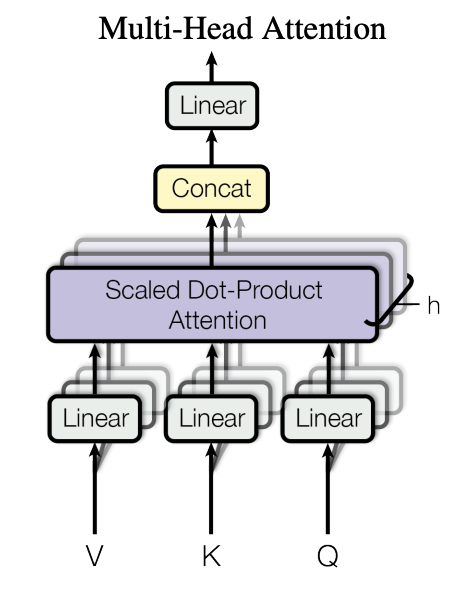
\includegraphics[width=0.5\textwidth]{ma.png}
	\caption{多头注意力的架构。多头注意力特征由h个缩放点乘注意力特征拼接得到。}
	\label{ma}
\end{figure}

基于以上多头注意力机制的思想,本文分别使用三种注意力特征:图片的自注意力(V-SA)、问题文本的自注意力(Q-SA)、由问题引导的对图像的注意力(GA)。假设文本词向量矩阵为$Y$,图像特征图为$X$,则在计算V-SA时,$Q = K = V = X$,即输出的图像特征为$SA=MA(X, X, X)$;在计算Q-SA时,$Q = K = V = Y$,即输出的文本特征为$SA=MA(Y, Y, Y)$;在计算引导注意力特征时,$Q = Y$为词向量矩阵,$K = V = X$为图像特征矩阵,并且词向量和图像特征向量具有相同的维度,即输出的由问题引导的图像特征为$GA=MA(Y, X, X)$。三种注意力组合的结构构成一个共同注意力模块(MCA),结构如图\ref{mca}。共同注意力模块以输入为原始的图像特征和文本特征,输出为经过注意力机制的图像和文本特征。
\begin{figure}[H]
	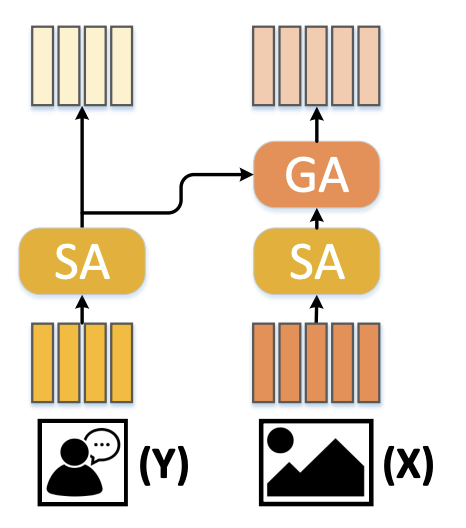
\includegraphics[width=0.3\textwidth]{mca.png}
	\caption{共同注意力模块(MCA)由一个V-SA、一个Q-SA和一个GA组成。}
	\label{mca}
\end{figure}

为了提高使用深度的注意力机制提取更高层次的特征,MCAN论文\citing{Yu_2019_CVPR}提出了Encoder-Decoder和Stacking两种级联MCA层的方式,如图\ref{mca_stacking}。
\begin{figure}[H]
	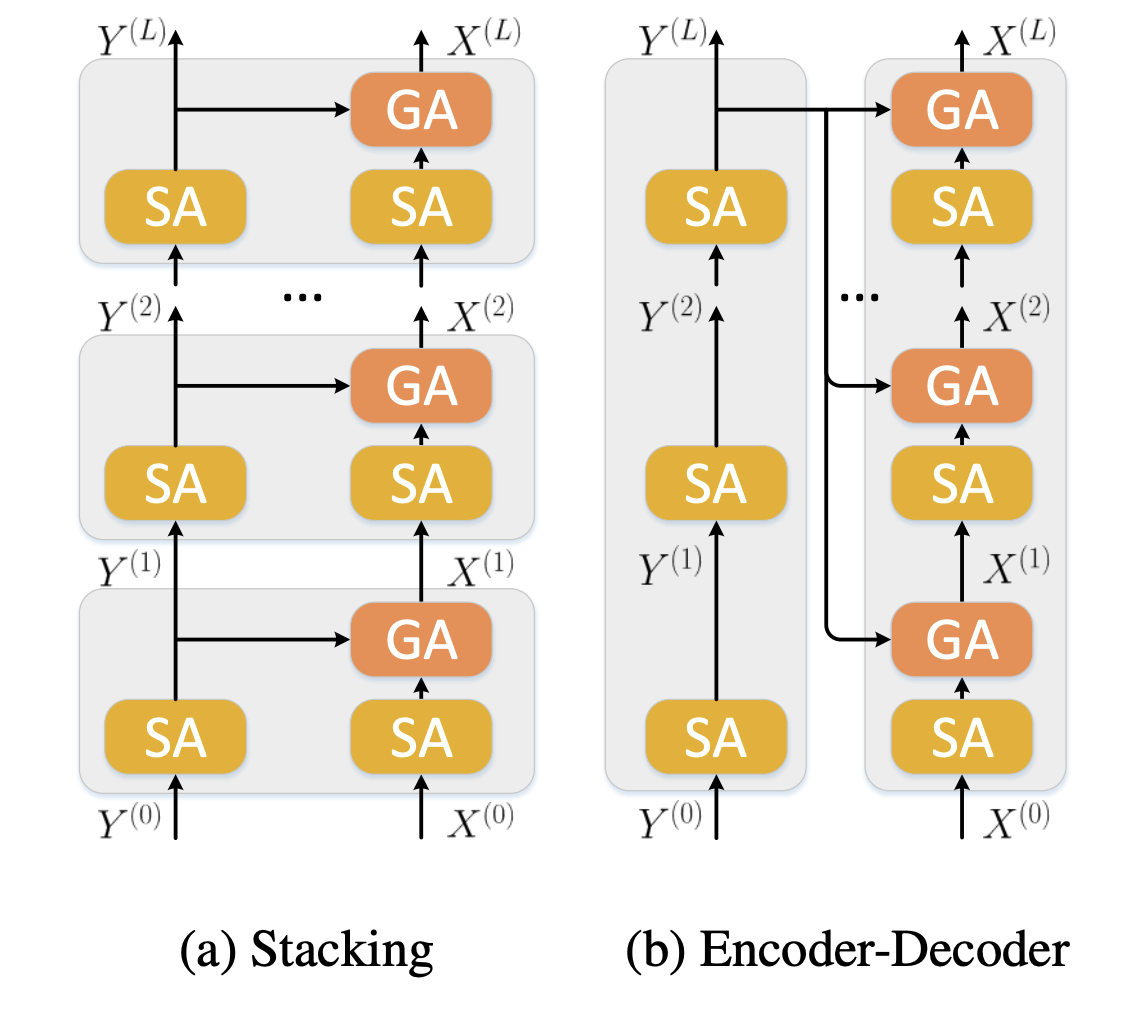
\includegraphics[width=0.5\textwidth]{mca_stacking.png}
	\caption{两种MCA层的级联方式,Stacking将上一层的输出直接作为下一层的输入,Encoder-Decoder将最后一层的问题自注意力特征作为每一层图像的查询矩阵。}
	\label{mca_stacking}
\end{figure}

根据文章给出的两种级联方式在多个任务的表现情况\citing{Yu_2019_CVPR},在本文中,我们使用Encoder-Decoder的级联方式,假定$SA^1$,$SA^2$,...,$SA^L$表示不同层的自注意力,$GA^1$,$GA^2$,...,$GA^L$表示不同层的引导注意力,$X^{(k)}$和$Y^{(k)}$分别表示第k层输出的图像特征和文本特征。因此第k层Encoder-Decoder级联的注意力模块的公式为,
\begin{equation}
Y^{(k)} = SA^{(k)}(Y^{(k-1)})
\end{equation}
\begin{equation}
X^{(k)} = GA^{(k)}(Y^{(L)}, SA^{(k)}(X^{(k-1)}))
\end{equation}
其中图像特征$X^{(0)}=X$,$Y^{(0)}=Y$。

在获得经过多层注意力的图像特征$X^{(L)}=[x^{(L)}_1,...,x^{(L)}_m]\in\mathbb{R}^{m \times d}$和文本特征$Y^{(L)}=[y^{(L)}_1,...,y^{(L)}_n]\in\mathbb{R}^{n \times d}$,我们对所有分量权重求和,进一步得到最终的图像特征$x$和文本特征$y$。以图像特征为例,公式如下。
\begin{equation}
\alpha = softmax(MLP(X^{(L)}))
\end{equation}
\begin{equation}
x = \sum_{i=1}^m \alpha_i x_i^{(L)}
\end{equation}
其中$\alpha = [\alpha_1,...,\alpha_m]$是图像特征分量的权重。

$Y^{(L)}$的计算方式类似。我们使用一下公式融合两种特征。
\begin{equation}
z = LayerNorm(W_x^Tx + W_y^Ty)
\end{equation}
其中$W_x, W_y \in \mathbb{R}^{d \times d_z}$是线性映射矩阵,$d_z$是融合后的特征向量的维度。最后我们使用softmax函数计算融合特征在$N$个类别的答案,$N$为训练集中出现频率最高的答案。最后我们使用交叉熵更新模型参数。

\section{实验}
为了确定不同的参数配置对于N-KBSN模型在视觉问答任务上的表现,我们使用通用的开放型问答数据集VQA2.0\citing{goyal2017making}训练模型,并和目前的最优模型性能进行比较分析。

\subsection{实验设置}
\textbf{数据集}\ 我们使用VQA2.0数据集训练模型。按照VQA挑战中的划分标准将数据集分为train/val/test三个数据子集,它们分别包含8万图像+44.4万问答对、4万图像+21.4万问答对、8万图像+44.8万问答对。答案包含“是否”、“数量”和“其他”三种类型,图片均为从MS-COCO数据集中提取的真实场景。此外,根据同时存在于VQA2.0和Visual Genome中的图片,我们还使用了从Visual Genome中提取出49万个问答对,用于增强训练集。

\textbf{超参数设置}\ 在文本中,输入的图像特征$x_i$的维度为2048,因此$X \in \mathbb{R}^{100 \times 2048}$。为衡量不同文本特征的性能表现,我们使用三种ELMO的参数配置,分别是$ELMO_s$/$ELMO_m$/$ELMO_l$,它们的参数量、LSTM的隐层大小、输出大小、$ELMo_k^{task}$大小见表\ref{ELMO_models}。我们使用一个线性层将elmo词向量统一转化为512维,融合特征$z \in \mathbb{R}^{1024}$。
\begin{table}[H]
% \resizebox{0.8\textwidth}{!}{}
\centering
\caption{三种 ELMO 的参数配置}
\begin{tabular*}{0.9\textwidth}{lp{2.5cm}p{2.5cm}p{2.5cm}p{2.5cm}}
\toprule
\textbf{Model} & \textbf{Parameters (Millions)} & \textbf{LSTM Size} & \textbf{Output Size} & \textbf{ELMO Size}\\
\midrule
$ELMO_s$&  13.6& 1024&  128& 256\\
$ELMO_m$&  28.0& 2048&  256& 512\\
$ELMO_l$&  93.6& 4096&  512& 1024\\
\bottomrule
\end{tabular*}
\label{ELMO_models}
\end{table}

多头注意力中的隐层维度为512,头数$h=8$,因此每个头的隐层维度$d_h=d/h=64$。根据\citing{teney2018tips}的建议,我们将答案词典大小设为$N=3129$。MCA层数$L$设为6;优化器Adam参数为$\beta_1=0.9$、$\beta_2=0.98$;学习率为$min(2.5te^{-5}, 1e^{-4})$,t为训练的epoch数;batch大小为64。

\subsection{剔除研究}
\subsection{实验结果分析}

\section{本章小结}

